% --- [ Performance ] ----------------------------------------------------------

\subsection{Performance}

% TODO: Rewrite, cleanup and verify (especially the \theta(...) claims!).

\textbf{NOTE}: \textit{The following paragraph is more of a brain-dump. It will be used as a basis for a future rewrite.}

Profiling was put to good use when optimizing the lexer, the code base of which is rather straight forward. When estimating the runtime complexity of the subgraph isomorphism search algorithm however the use of intuition and algorithm research was far more valuable. For this specific task the generic problem (subgraph isomorphism search of arbitrary input graphs) could be simplified (TODO: use generalized instead of simplified?) to a much easier problem as every node of the graph were known to be connected (TODO: find the succinct term in graph theory to express this concept). Exploiting this property lead to an algorithm that had a runtime complexity of $ \Theta(n*m) $ where $ m $ is known to be small rather than $ \Theta(n^m) $ as is the case for a brute force algorithm and $ \Theta(n^log(m)) $ (TODO: Find the correct runtime complexity of the Hillman iso search algo) as was the case of the Hillman subgraph isomorphism search algorithm which is capable of solving the generic case, improving on the brute force approach by applying heuristics (TODO: is heuristics the right word to use here?) to prune the search space.

In summary, using profiling is great for simple problems. Using algorithm research, runtime complexity theory and intuition is needed for complex problems. Knowledge about specific properties of the problem which may be exploited.

foo

% --- [ Subsubsections ] -------------------------------------------------------

% ~~~ [ Profiling ] ~~~~~~~~~~~~~~~~~~~~~~~~~~~~~~~~~~~~~~~~~~~~~~~~~~~~~~~~~~~~

\subsubsection{Profiling}
\label{sec:ver_profiling}

The initial implementation of the LLVM IR lexer (see section \ref{sec:impl_llvm_ir_library}) focused on correctness, and strived to be as simple and straight forward as possible. Once feature complete and thoroughly tested, the lexer was profiled for the first time and a major performance bottleneck was identified; as illustrated in figure \ref{fig:lexer_pprof}. When scanning letters, the \texttt{lexLetter} function used a hash map to check if the scanned letters were part of a keyword. As letters make up the majority of the characters in LLVM IR source files, this caused an extensive number of hash map iterations which accounted for roughly 70\% of the total execution time. To fix this issue, a benchmark test was implemented to measure the performance changes between the original and the updated version; as further described in section \ref{sec:ver_benchmarks}. At this stage, only CPU profiling has been utilized to identify performance bottlenecks. Future work may leverage memory profiling to further improve the performance of the decompilation components.

\begin{figure}[htbp]
	\begin{center}
		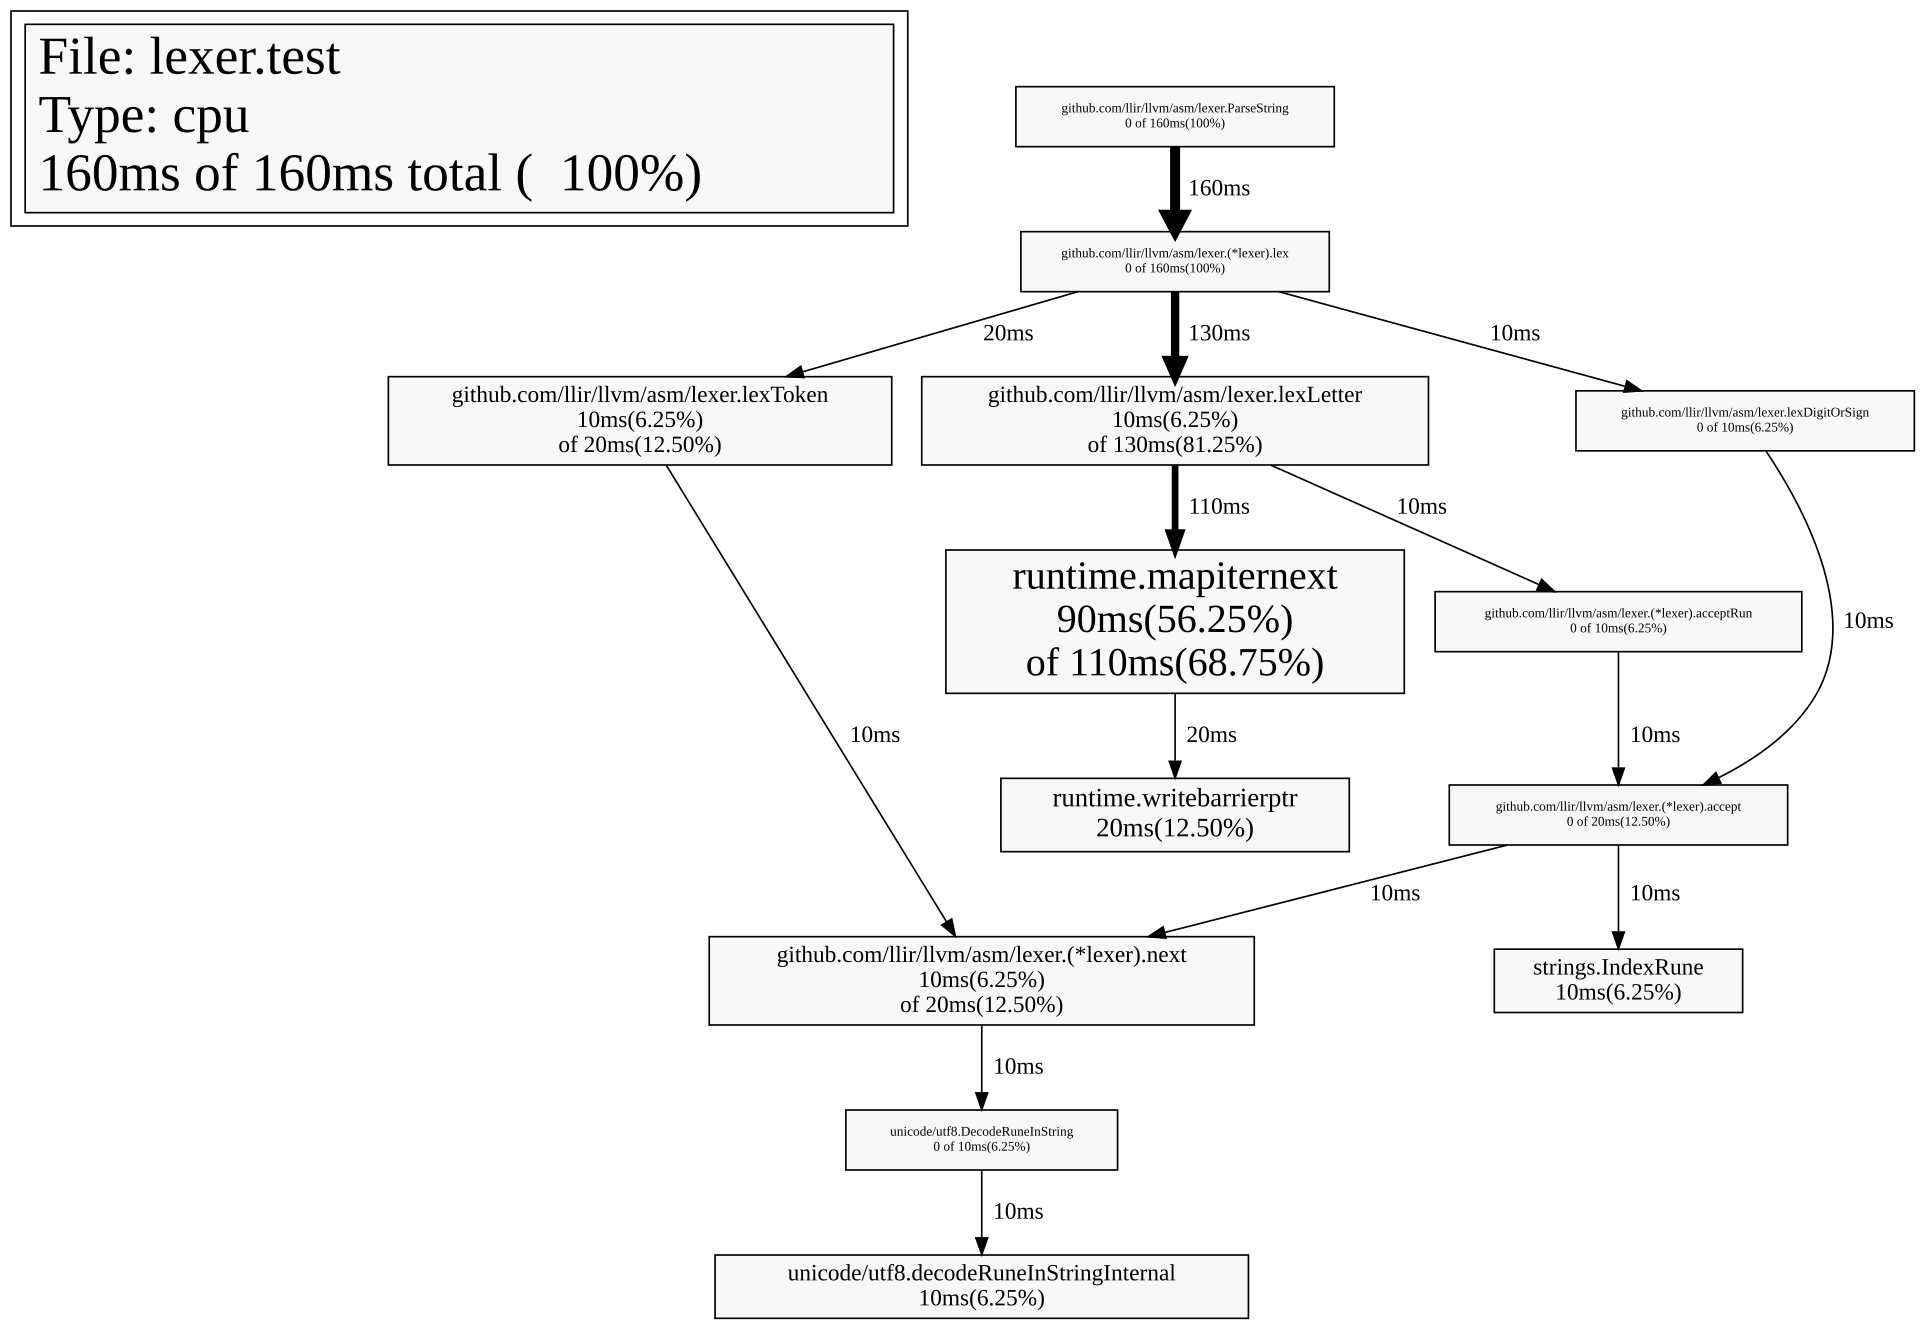
\includegraphics[width=\textwidth]{inc/8_ver/lexer_pprof.png}
		\caption{A major performance bottleneck was located when profiling the LLVM IR lexer for the first time. Roughly 70\% of the total execution time was spent doing hash map iterations (i.e. \texttt{runtime.mapiternext}).}
		\label{fig:lexer_pprof}
	\end{center}
\end{figure}

% ~~~ [ Benchmarks ] ~~~~~~~~~~~~~~~~~~~~~~~~~~~~~~~~~~~~~~~~~~~~~~~~~~~~~~~~~~~

\subsubsection{Benchmarks}
\label{sec:ver_benchmarks}

Benchmark tests were implemented to reliably measure any performance changes before trying to resolve performance issues. An updated version of the LLVM IR library used arrays instead of hash maps to identify keywords when scanning letters, which resolved the performance issue identified in section \ref{sec:ver_profiling}. The updated version of the LLVM IR lexer is roughly 3.6 times faster than the original version, as illustrated in figure \ref{fig:benchmark_delta}.

\begin{figure}[htbp]
	\begin{center}
		\begin{verbatim}
$ git checkout old; go test -bench=ParseString > old.txt
$ git checkout new; go test -bench=ParseString > new.txt
$ benchcmp old.txt new.txt
benchmark                old ns/op     new ns/op     delta
BenchmarkParseString     737625        204010        -72.34%
		\end{verbatim}
		\caption{Benchmark run time delta between the original and the optimized version of the LLVM IR lexer, as visualized by \texttt{benchcmp}\protect\footnotemark. The optimized version is roughly 3.6 times faster than the original vesion of the lexer.}
		\label{fig:benchmark_delta}
	\end{center}
\end{figure}
\footnotetext{Benchcmp displays performance changes between benchmarks: \url{https://golang.org/x/tools/cmd/benchcmp}}

